%!LW recipe=pdflatex -> bibtex -> pdflatex -> pdflatex
\documentclass[conference, letterpaper]{IEEEtran}
\usepackage{cite}
\usepackage{amsmath,amssymb,amsfonts}
\usepackage{algorithmic}
\usepackage{graphicx}
\usepackage{textcomp}
\usepackage{xcolor}
\usepackage{blindtext}
\usepackage{booktabs}
\usepackage{bm}

\def\BibTeX{{\rm B\kern-.05em{\sc i\kern-.025em b}\kern-.08em
    T\kern-.1667em\lower.7ex\hbox{E}\kern-.125emX}}
\begin{document}

\title{Biomechanical Analysis of Chicken Ulna and Radius: A Comparative Study of Three-Point and Four-Point Bending}

\author{\IEEEauthorblockN{Jamie Kang}}

\maketitle

\section{Introduction}
    This experiment delves into the mechanical properties of chicken bones through three-point and four-point bending tests. Bones, with their intricate internal and external structures, exhibit unique bending behaviors, particularly in response to lever-like forces. The objective is to characterize how these bones respond to bending loads, offering insights into the mechanical interactions of their cortical and cancellous components. The hypothesis posits that geometric details, such as cortical thickness and cancellous distribution, intricately influence the bones' bending behavior. By connecting the experiment to bone anatomy and biomechanics, this study seeks to unravel the nuanced relationship between bone structure and mechanical response.

\section{Materials and Methods}
    Two chicken bones, the radius and ulna, underwent three-point (ulna) and four-point (radius) bending tests using the CellScale UniVert compression tester following the lab manual~\cite{3LM2023}. The machine was set up with a template, and the bones were positioned symmetrically between supports. Load cell zeroing and image documentation preceded test execution. Moment of inertia (MOI) was calculated using a caliper and ellipse approximation. In addition to the collected data, image analysis in SolidWorks and data analysis from previous Sawbone samples informed the generation of force-displacement plots, identification of linear regions, and the calculation of Young's modulus and ultimate stress for both bending configurations.

\section{Results}
    Sample calculations for Sawbone test result values can be found in Appendix~\ref{apdx_a}.
    \begin{figure}[htbp]
        \centerline{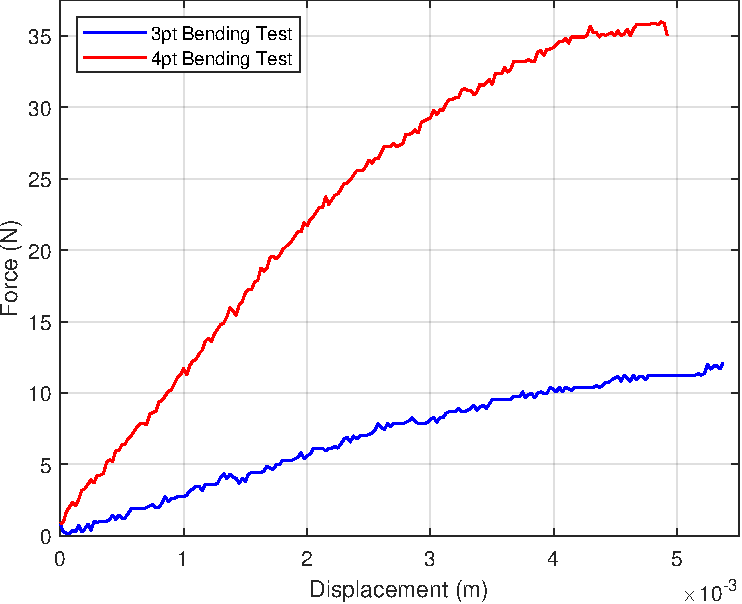
\includegraphics[width = 0.65\linewidth]{sawbones_fd.pdf}}
        \caption{Plot of force vs.\ displacement for both Sawbone bending tests.}\label{sawbones_fd}
    \end{figure}
    \vspace*{-\baselineskip}
    \begin{figure}[htbp]
        \centerline{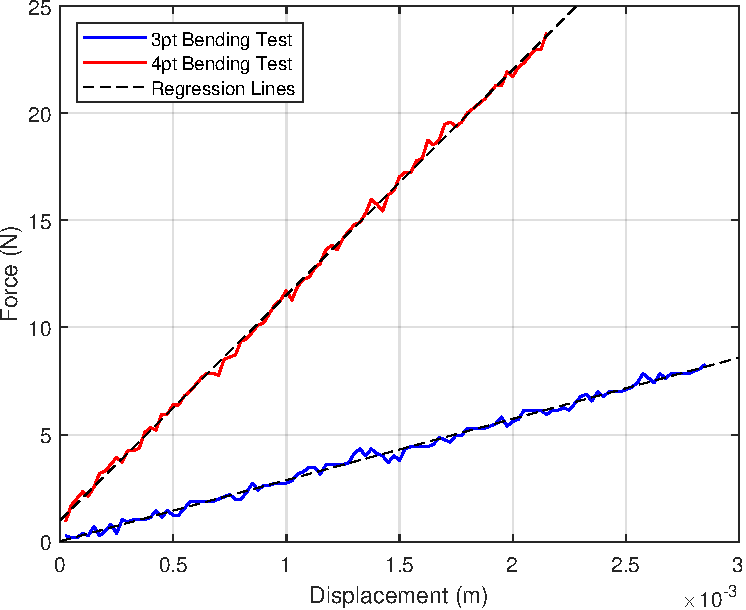
\includegraphics[width = 0.65\linewidth]{sawbones_linear.pdf}}
        \caption{Plot of the linear regions of force vs.\ displacement for both Sawbone bending tests.}\label{sawbones_linear}
    \end{figure}
    \begin{table}[htbp]
        \caption{Sawbone Sample Results}
        \begin{minipage}{\linewidth}
            \centering
            \begin{tabular}{lcc}
                \toprule{}
                & \textbf{3-Point Bending} & \textbf{4-Point Bending} \\
                \midrule{}
                \hspace*{-1ex}\textbf{Young's Modulus (E)} & \(1.4325\ \text{MPa}\)  & \(11.4963\ \text{MPa}\)  \\
                \textbf{Ultimate Stress (\(\bm{\sigma_u}\))} & \(145.5435\ \text{kPa}\)  & \(338.5217\ \text{kPa}\)  \\
                \textbf{MOI} & \(7.2115\times10^{-9}\ \text{m}^4\)  & \(4.9426\times10^{-9}\ \text{m}^4\)  \\
                \midrule{}
                \hspace*{-1ex}\textbf{\% Difference MOI} & \multicolumn{2}{c}{37.3346 \%} \\
                \bottomrule{}
            \end{tabular}\label{tbl_1}
            \vspace*{-\baselineskip}
        \end{minipage}
    \end{table}
    \begin{figure}[htbp]
        \centerline{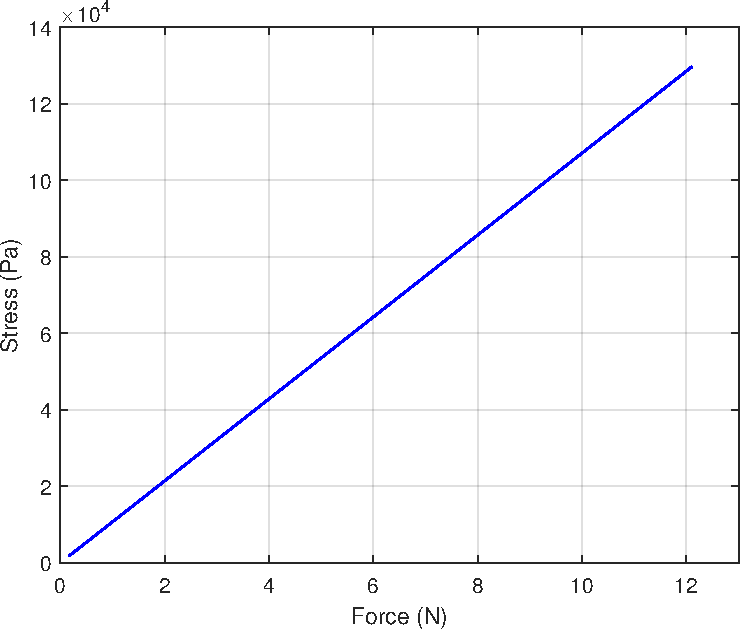
\includegraphics[width = 0.65\linewidth]{sawbones_sf.pdf}}
        \caption{Plot of stress vs.\ load for 3-point Sawbone bending test.}\label{sawbones_sf}
    \end{figure}
    \begin{figure}[htbp]
        \centerline{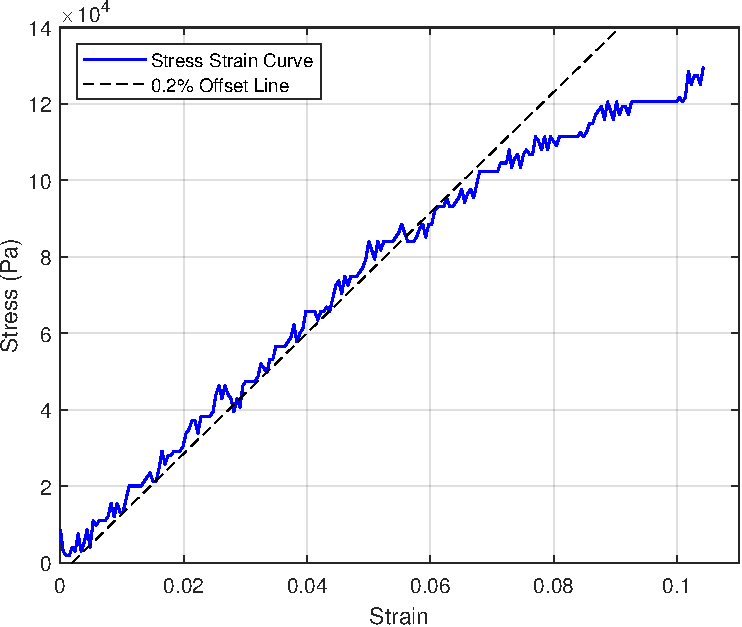
\includegraphics[width = 0.65\linewidth]{sawbones_ss.pdf}}
        \caption{Plot of stress vs.\ strain for 3-point Sawbone bending test.}\label{sawbones_ss}
    \end{figure}
    \begin{figure}[htbp]
        \centerline{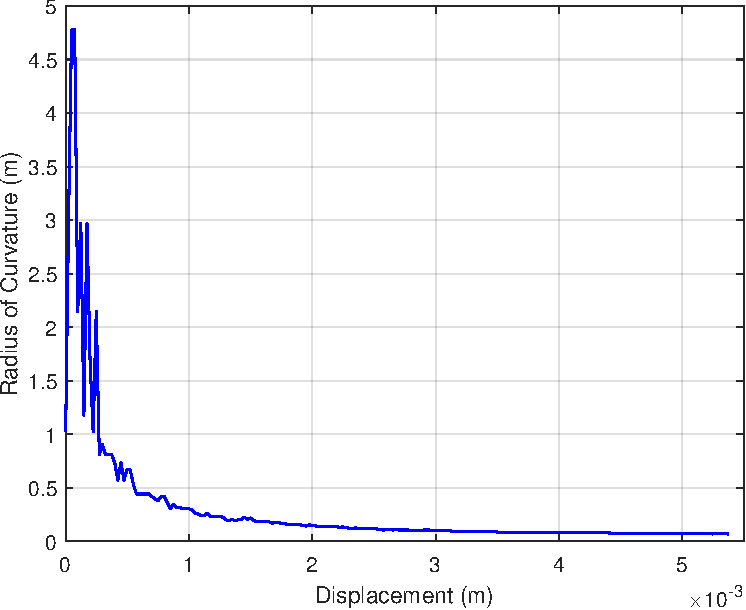
\includegraphics[width = 0.65\linewidth]{sawbones_rd.pdf}}
        \caption{Plot of radius of curvature vs.\ displacement for 3-point Sawbone bending test.}\label{sawbones_rd}
    \end{figure}

    Sample calculations for radius and ulna test result values can be found in Appendix~\ref{apdx_b}.
    \begin{figure}[htbp]
        \centerline{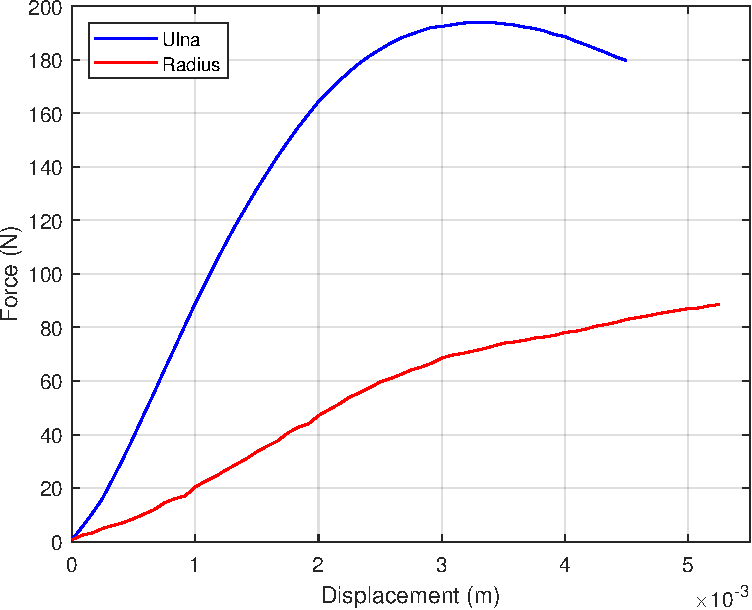
\includegraphics[width = 0.65\linewidth]{chicken_fd.pdf}}
        \caption{Plot of force vs.\ displacement for both chicken bone bending tests.}\label{chicken_fd}
    \end{figure}
    \begin{figure}[htbp]
        \centerline{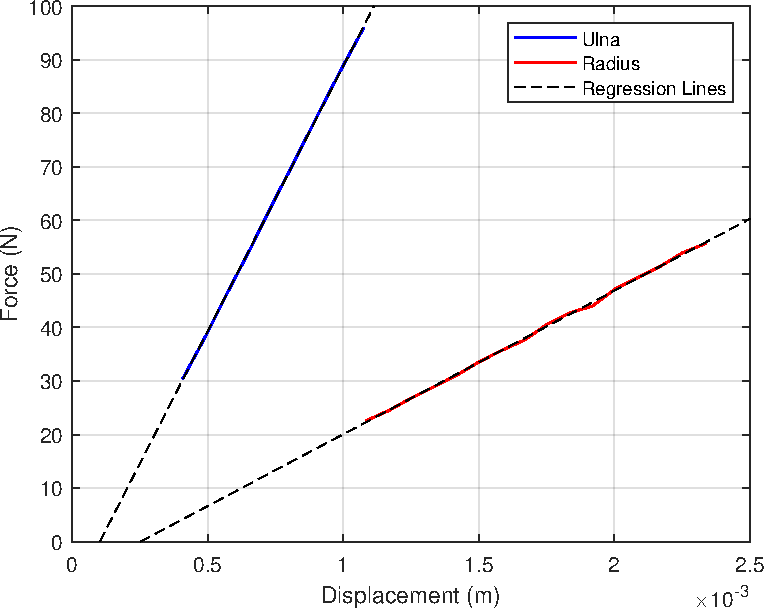
\includegraphics[width = 0.65\linewidth]{chicken_linear.pdf}}
        \caption{Plot of the linear regions of force vs.\ displacement for both chicken bone bending tests.}\label{chicken_linear}
    \end{figure}

    \begin{table}[htbp]
        \caption{Ulna and Radius Results Using the Ellipse Approximation Method and Image Analysis Method}
        \begin{minipage}{\linewidth}
            \centering
            \begin{tabular}{lcc}
                \toprule{}
                & \textbf{Ulna} & \textbf{Radius} \\
                \midrule{}
                \hspace*{-1ex}\textbf{MOI\textsubscript{image}} & \(71.23\ \text{mm}^4\) & \(16.26\ \text{mm}^4\) \\
                \textbf{MOI\textsubscript{ellipse}} & \(24.553\ \text{mm}^4\) & \(7.2942\ \text{mm}^4\) \\
                \textbf{\% Difference MOI} & \(97.464\ \text{\%}\) & \(76.1293\ \text{\%}\) \\
                \midrule{}
                \hspace*{-1ex}\textbf{Young's Modulus (E)\textsubscript{image}} & \(5.0289\ \text{GPa}\) & \(8.9242\ \text{GPa}\) \\
                \textbf{Young's Modulus (E)\textsubscript{ellipse}} & \(14.5891\ \text{GPa}\) & \(19.8935\ \text{GPa}\) \\
                \textbf{\% Difference E} & \(97.464\ \text{\%}\) & \(76.1293\ \text{\%}\) \\
                \midrule{}
                \hspace*{-1ex}\textbf{Ultimate Stress (\(\bm{\sigma_u}\))\textsubscript{image}} & \(108.6298\ \text{MPa}\) & \(109.4894\ \text{MPa}\) \\
                \textbf{Ultimate Stress (\(\bm{\sigma_u}\))\textsubscript{ellipse}} & \(315.1427\ \text{MPa}\) & \(244.0707\ \text{MPa}\) \\
                \textbf{\% Difference \(\bm{\sigma_u}\)} & \(97.464\ \text{\%}\) & \(76.1293\ \text{\%}\) \\
                \bottomrule{}
            \end{tabular}\label{tbl_2}
            \vspace*{-\baselineskip}
        \end{minipage}
    \end{table}

\section{Discussion}
    Rotating the Sawbone specimen by 90° in a three-point bending experiment alters geometric parameters, affecting bending stiffness and MOI, while leaving material-specific properties like Young's modulus and ultimate stress unaffected. Applying the 0.2\% offset method in the three-point bending test predicted the Sawbone specimen's yield stress for a tensile test, yielding 85.1897 kPa. This method correlates with tension in a uniaxial test. The flexure formula calculates the constant radius of curvature (R) across the beam length under linear elastic bending, observed in Fig.~\ref{sawbones_rd}. In four-point bending, the UniVert machine's limitations influenced support distance choices, impacting load application and machine load capacity.

    Three-point bending induces uniform stress along the beam, resulting in a single peak bending moment, while four-point bending introduces complexity, illustrated in Fig. 5 of~\cite{Xue2017}, potentially causing two-point fractures. Our experiment showed single-point fractures, but varied results exist. Three-point bending suits initial material characterization, while four-point bending delves into material behavior intricacies and potential weak points.

    Bones exhibit varying strengths in tension and compression, crucial for resisting bending loads and fractures~\cite{Takata2011}. Cortical bone provides compression strength, while cancellous bone absorbs energy and deforms during loading~\cite{Dai2022}. Comparing image analysis and ellipse approximation for moment of inertia (MOI) calculations involves accuracy versus practicality trade-offs. Image analysis is meticulous but requires specialized software, while the ellipse method simplifies irregular bone shapes quickly.

    Experimental results in Table~\ref{tbl_1} and Table~\ref{tbl_2} reveal material differences. The ulna's higher MOI suggests greater bending resistance, aligning with its forearm stability role~\cite{Lu2012}. The radius's higher Young's Modulus signifies increased stiffness, ideal for rotational movements like pronation and supination~\cite{Shaaban2006}. These adaptations align with distinct biomechanical roles of the ulna and radius in the forearm.

\bibliographystyle{ieeetran}
\bibliography{lab3}

\appendices{}
    \section{Sample Calculations for Sawbones}\label{apdx_a}
        \subsection{MOI --- 3pt}\label{apdx_aa}
            Moment of inertia about x-axis~\cite{Hibbeler2022}:
            \begin{align*}
                I_x
                &= \frac{1}{12}ba^3 \\
                &= \frac{1}{12}\left(0.00751\ \text{m}\right){\left(0.01243\ \text{m}\right)}^3 \\
                &= 7.2115\times10^{-9}\ \text{m}^4
            \end{align*}

        \subsection{Young's Modulus --- 3pt}\label{apdx_ab}
            The maximum deflection equation for three-point bending~\cite{3LM2023} is as follows:
            \begin{align}\label{eqn:slope3}
                \delta_{\max}
                = \frac{PL^3}{48E{I_x}}
                \implies 
                \frac{P}{\delta_{\max}}
                = \frac{48E{I_x}}{L^3}
            \end{align}
            The slope of the linear region of the force vs.\ displacement curve \(\frac{P}{\delta_{\max}}\) was found using the \texttt{polyfit} function in MATLAB:\@
            \[
                \frac{P}{\delta_{\max}} 
                = 2853.9519\ \text{N}
                = 2.8540\ \text{kN}
            \]
            Plugging in known values into~\eqref{eqn:slope3}:
            \begin{align*}
                (2853.9519\ \text{N})
                &= \frac{48E(7.2115\times10^{-9}\ \text{m}^4)}{{(0.0558\ \text{m})}^3}\\
                E 
                &= 1432467.1787\ \text{Pa}
                = 1.4325\ \text{MPa}
            \end{align*}

        \subsection{Young's Modulus --- 4pt}\label{apdx_ac}
            The displacement equation along the shaft in four-point bending~\cite{3LM2023} is as follows:
            \begin{align*}
                &\delta (x) \\
                &= \frac{P(L-a)}{6LE{I_x}}
                \left[ \frac{L}{L-a} {(x-a)}^3 - x^3 + (L^2 - {(L-a)}^2)x \right] \\
                &\quad + \frac{Pa}{6LE{I_x}}
                \left[ \frac{L}{a} {\left( x - (L-a) \right) }^3 - x^3 + (L^2 - a^2)x \right]
            \end{align*}
            Plugging in \(L = 0.05946\) m and \(a = 0.0201\) m:
            \begin{align*}
                \delta (a)
                &= \frac{P(0.11033)}{E{I_x}} \left( 3.1804\times10^{-5} \right) \\
                &\quad + \frac{P(0.05634)}{E{I_x}} \left( 3.3687\times10^{-5} \right) \\
                \delta (a) &= \frac{P}{E{I_x}} \left( 5.4067\times10^{-6} \right)
            \end{align*}
            The equation can then be rearranged as follows:
            \begin{equation}\label{eqn:slope4}
                \frac{P}{\delta (x)}
                = \frac{E{I_x}}{5.4067\times10^{-6}}
            \end{equation}
            The slope of the linear region of the force vs.\ displacement curve \(\frac{P}{\delta (x)}\) was found using the \texttt{polyfit} function in MATLAB:\@
            \[
                \frac{P}{\delta (x)} 
                = 10509.418\ \text{N}
                = 10.5194\ \text{kN}
            \]
            Plugging in known values into~\eqref{eqn:slope4}:
            \begin{align*}
                (10509.418\ \text{N})
                &= \frac{E(4.9426\times10^{-9}\ \text{m}^4)}{5.4067\times10^{-6}} \\
                E 
                &= 11496261.382\ \text{Pa}
                = 11.4963\ \text{MPa}
            \end{align*}

        \subsection{Ultimate Stress --- 3pt}\label{apdx_ad}
            Peak bending moment is observed at maximum load and at the farthest point from the neutral axis, thus \(c = \frac{a}{2} = 0.006215\ \text{m}\). The ultimate stress can then be found using the bending stress equation~\cite{Hibbeler2022}.
            \begin{align*}
                \vert \sigma _u \vert 
                &= \frac{Mc}{I_x} \\
                &= \frac{(0.16888\ \text{N}\cdot\text{m})(0.006215\ \text{m})}{(7.2115\times10^{-9}\ \text{m}^4)} \\
                &= 145543.4559\ \text{Pa}
                = 145.5435\ \text{kPa}
            \end{align*}

    \section{Sample Calculations for Chicken Bones}\label{apdx_b}
        \subsection{MOI Using Ellipse Approximation --- Ulna}\label{apdx_ba}
            As seen in Fig.~\ref{ulna_measurements}, measurements were taken in the orientation where bending occurs about the x-axis.
            \begin{figure}[htbp]
                \centerline{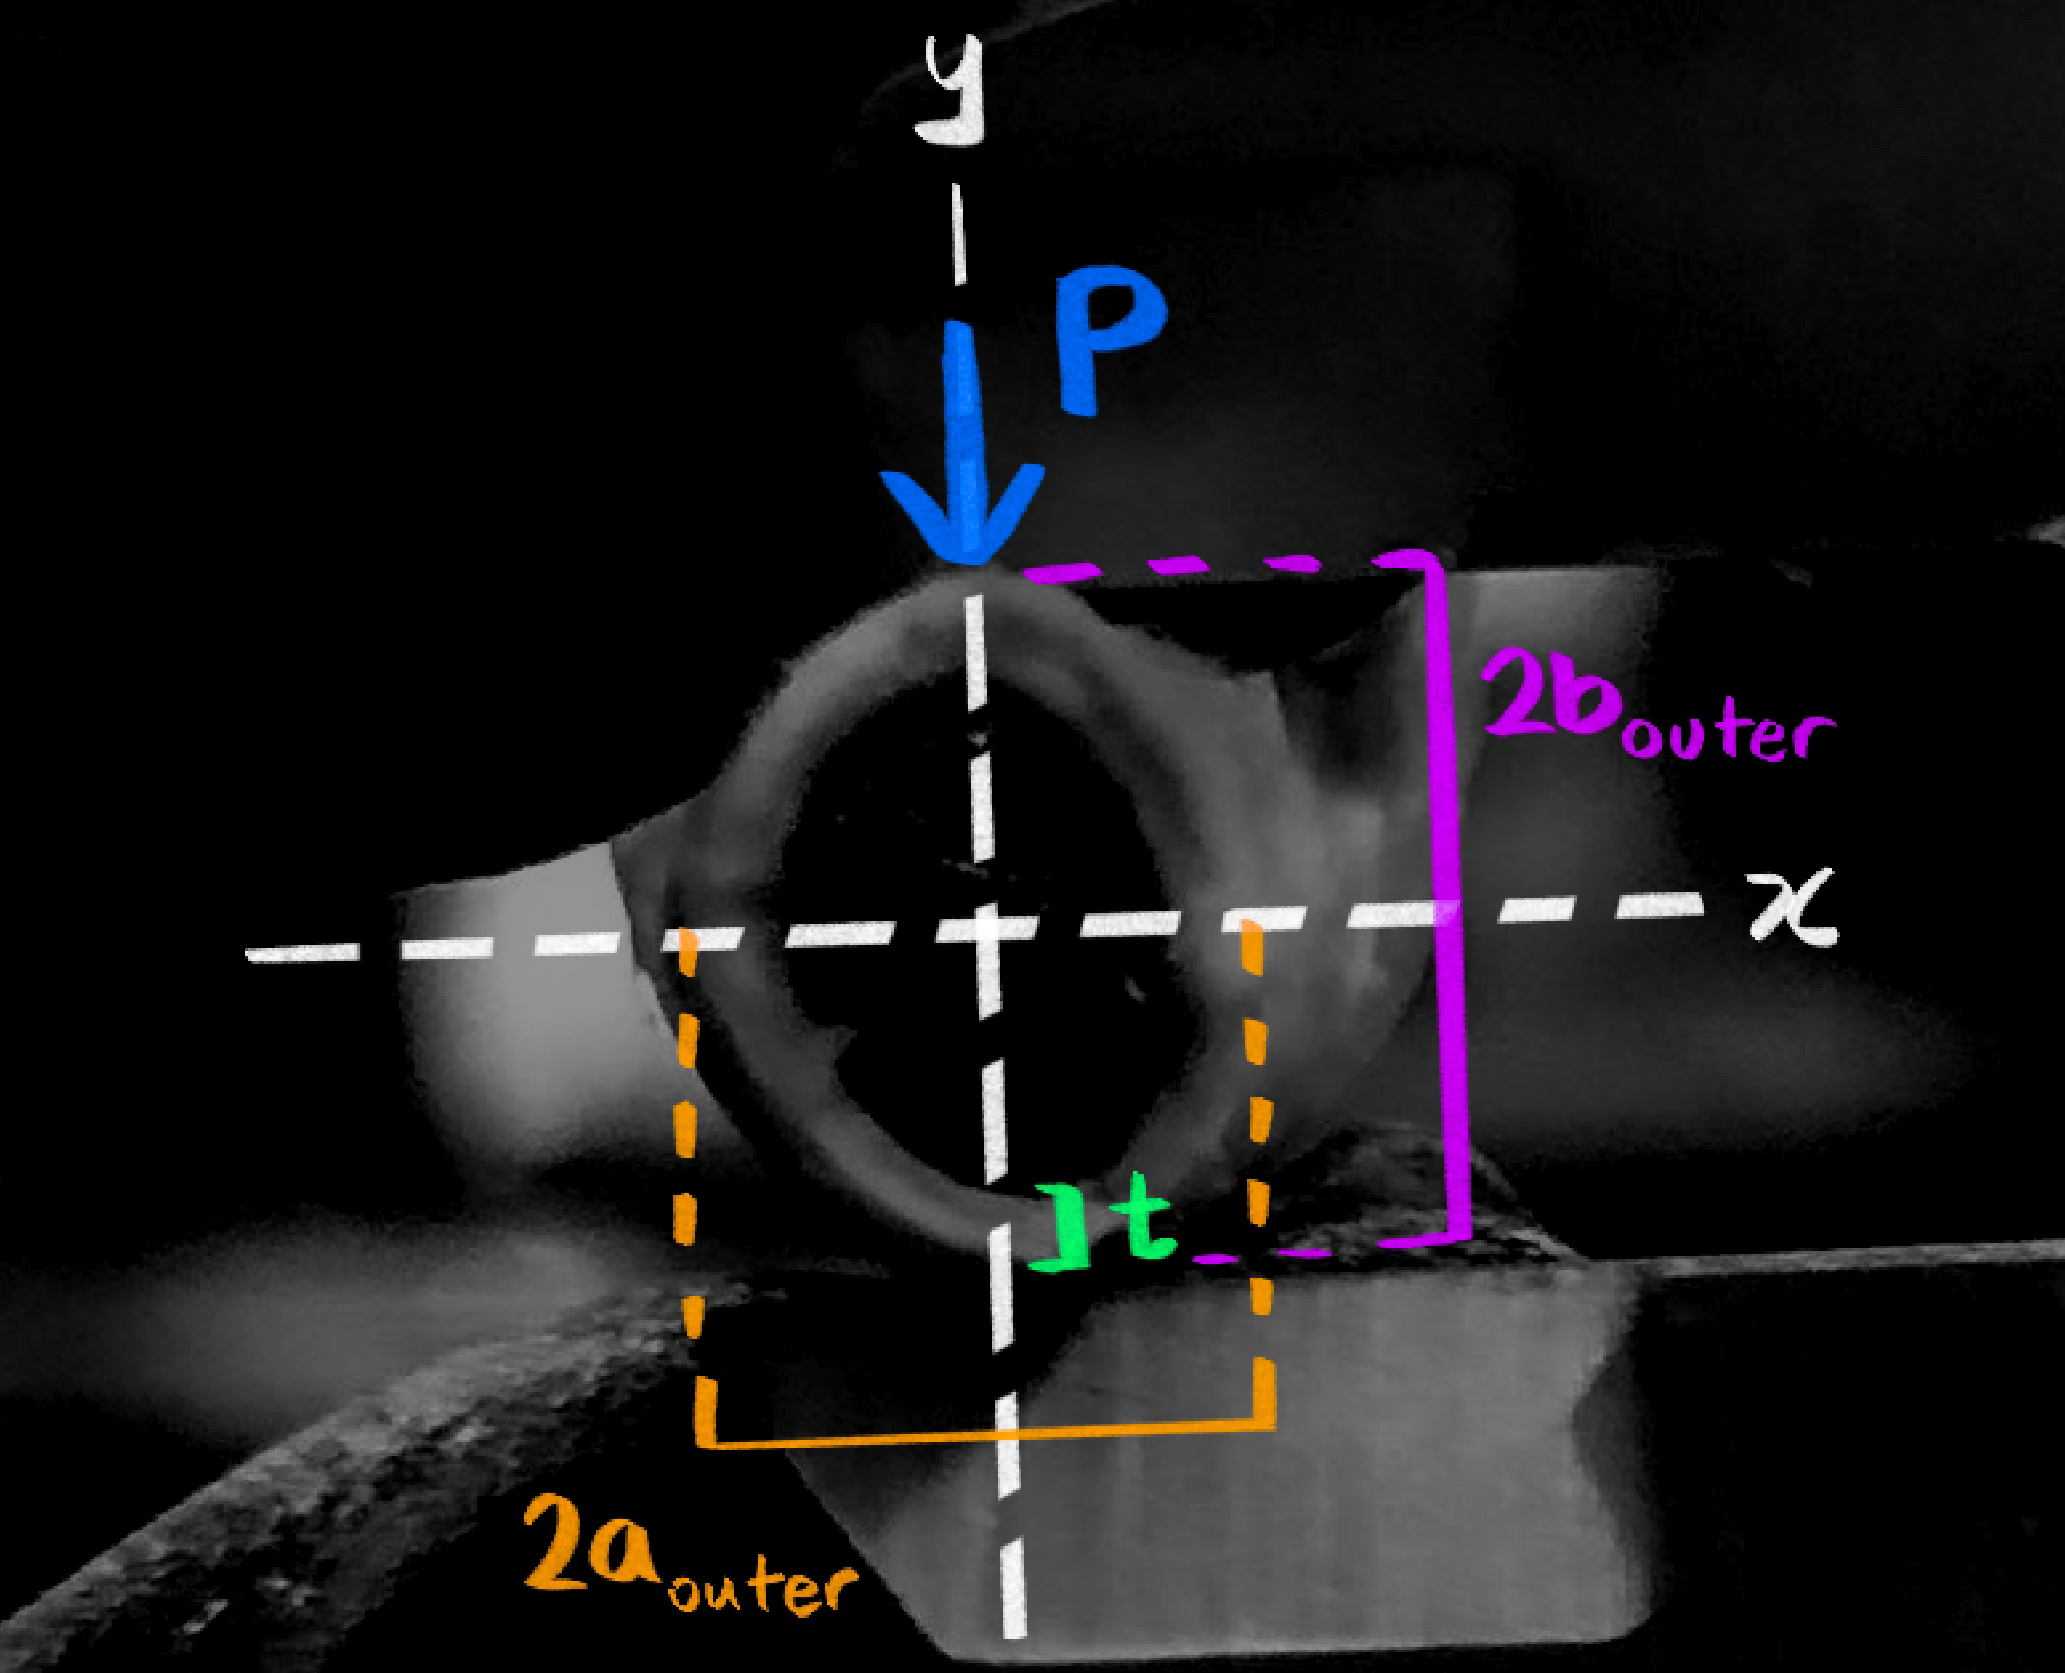
\includegraphics[width = 0.75\linewidth]{ulna_measurements.png}}
                \caption{Cross-section photo of ulna, with measurements taken labeled.}\label{ulna_measurements}
            \end{figure}
            
            \(a_{outer} = 0.0036\ \text{m}\), \(b_{outer} = 0.00286\ \text{m}\), and thickness \(t = 0.00066\ \text{m}\) measured were used to calculate values needed to calculate MOI:\@
            \begin{align*}
                a_{inner} &= a_{outer} - \frac{t}{2} = 0.00327\ \text{m}\\
                b_{inner} &= b_{outer} - \frac{t}{2} = 0.00253\ \text{m}
            \end{align*} 

            Using the equation of moment of inertia of an ellipse~\cite{3LM2023}, the inner and outer MOI was calculated to find the MOI of the hollow ellipse shape of the bone.
            \begin{align*}
                {(I_x)}_{outer}
                &= \frac{\pi (a_{outer}) {(b_{outer})}^3}{4} = 6.6144\times10^{-11}\ \text{m}^4\\
                {(I_x)}_{inner}
                &= \frac{\pi (a_{inner}) {(b_{inner})}^3}{4} = 4.1591\times10^{-11}\ \text{m}^4
            \end{align*}
            \[
                {(MOI)}_{ellipse} 
                = {(I_x)}_{outer} - {(I_x)}_{inner} 
                = 2.4553\times10^{-11}\ \text{m}^4
            \]
            
        \subsection{Young's Modulus --- Ulna}\label{apdx_bb}
            Following steps outlined in Appendix~\ref{apdx_ab}, the slope of the linear region of the force vs.\ displacement curve \(\frac{P}{\delta_{\max}}\) was found using the \texttt{polyfit} function in MATLAB once more:\@
            \[
                \frac{P}{\delta_{\max}} 
                = 98962.6626\ \text{N}
                = 98.9627\ \text{kN}
            \]
            Plugging in known values into~\eqref{eqn:slope3}:
            \begin{align*}
                (98962.6626\ \text{N})
                &= \frac{48E(7.123\times10^{-11}\ \text{m}^4)}{{(0.0558\ \text{m})}^3}\\
                E 
                &= 5028862791.3324\ \text{Pa}
                = 5.0289\ \text{GPa}
            \end{align*}

        \subsection{Young's Modulus --- Radius}\label{apdx_bc}
            Following steps outlined in Appendix~\ref{apdx_ac}, the slope of the linear region of the force vs.\ displacement curve \(\frac{P}{\delta (x)}\) was found using the \texttt{polyfit} function in MATLAB once more:\@
            \[
                \frac{P}{\delta (x)} 
                = 26838.1894\ \text{N}
                = 26.8382\ \text{kN}
            \]
            Plugging in known values into~\eqref{eqn:slope4}:
            \begin{align*}
                (26838.1894\ \text{N})
                &= \frac{E(7.123\times10^{-11}\ \text{m}^4)}{5.4067\times10^{-6}} \\
                E 
                &= 8924179123.0254\ \text{Pa}
                = 8.9242\ \text{GPa}
            \end{align*}

        \subsection{Ultimate Stress --- Ulna}\label{apdx_bd}
            Following steps outlined in Appendix~\ref{apdx_ad}, the ultimate stress is calculated using \(c = b_{outer} = 0.00286\ \text{m}\):\@
            \begin{align*}
                \vert \sigma _u \vert 
                &= \frac{Mc}{{(MOI)}_{image}} \\
                &= \frac{(2.7055\ \text{N}\cdot\text{m})(0.00286\ \text{m})}{(7.123\times10^{-11}\ \text{m}^4)} \\
                &= 108629846.6096\ \text{Pa}
                = 108.6298\ \text{MPa}
            \end{align*}

        \subsection{MOI Using Image Analysis --- Ulna}\label{apdx_be}
            \begin{figure}[htbp]
                \centerline{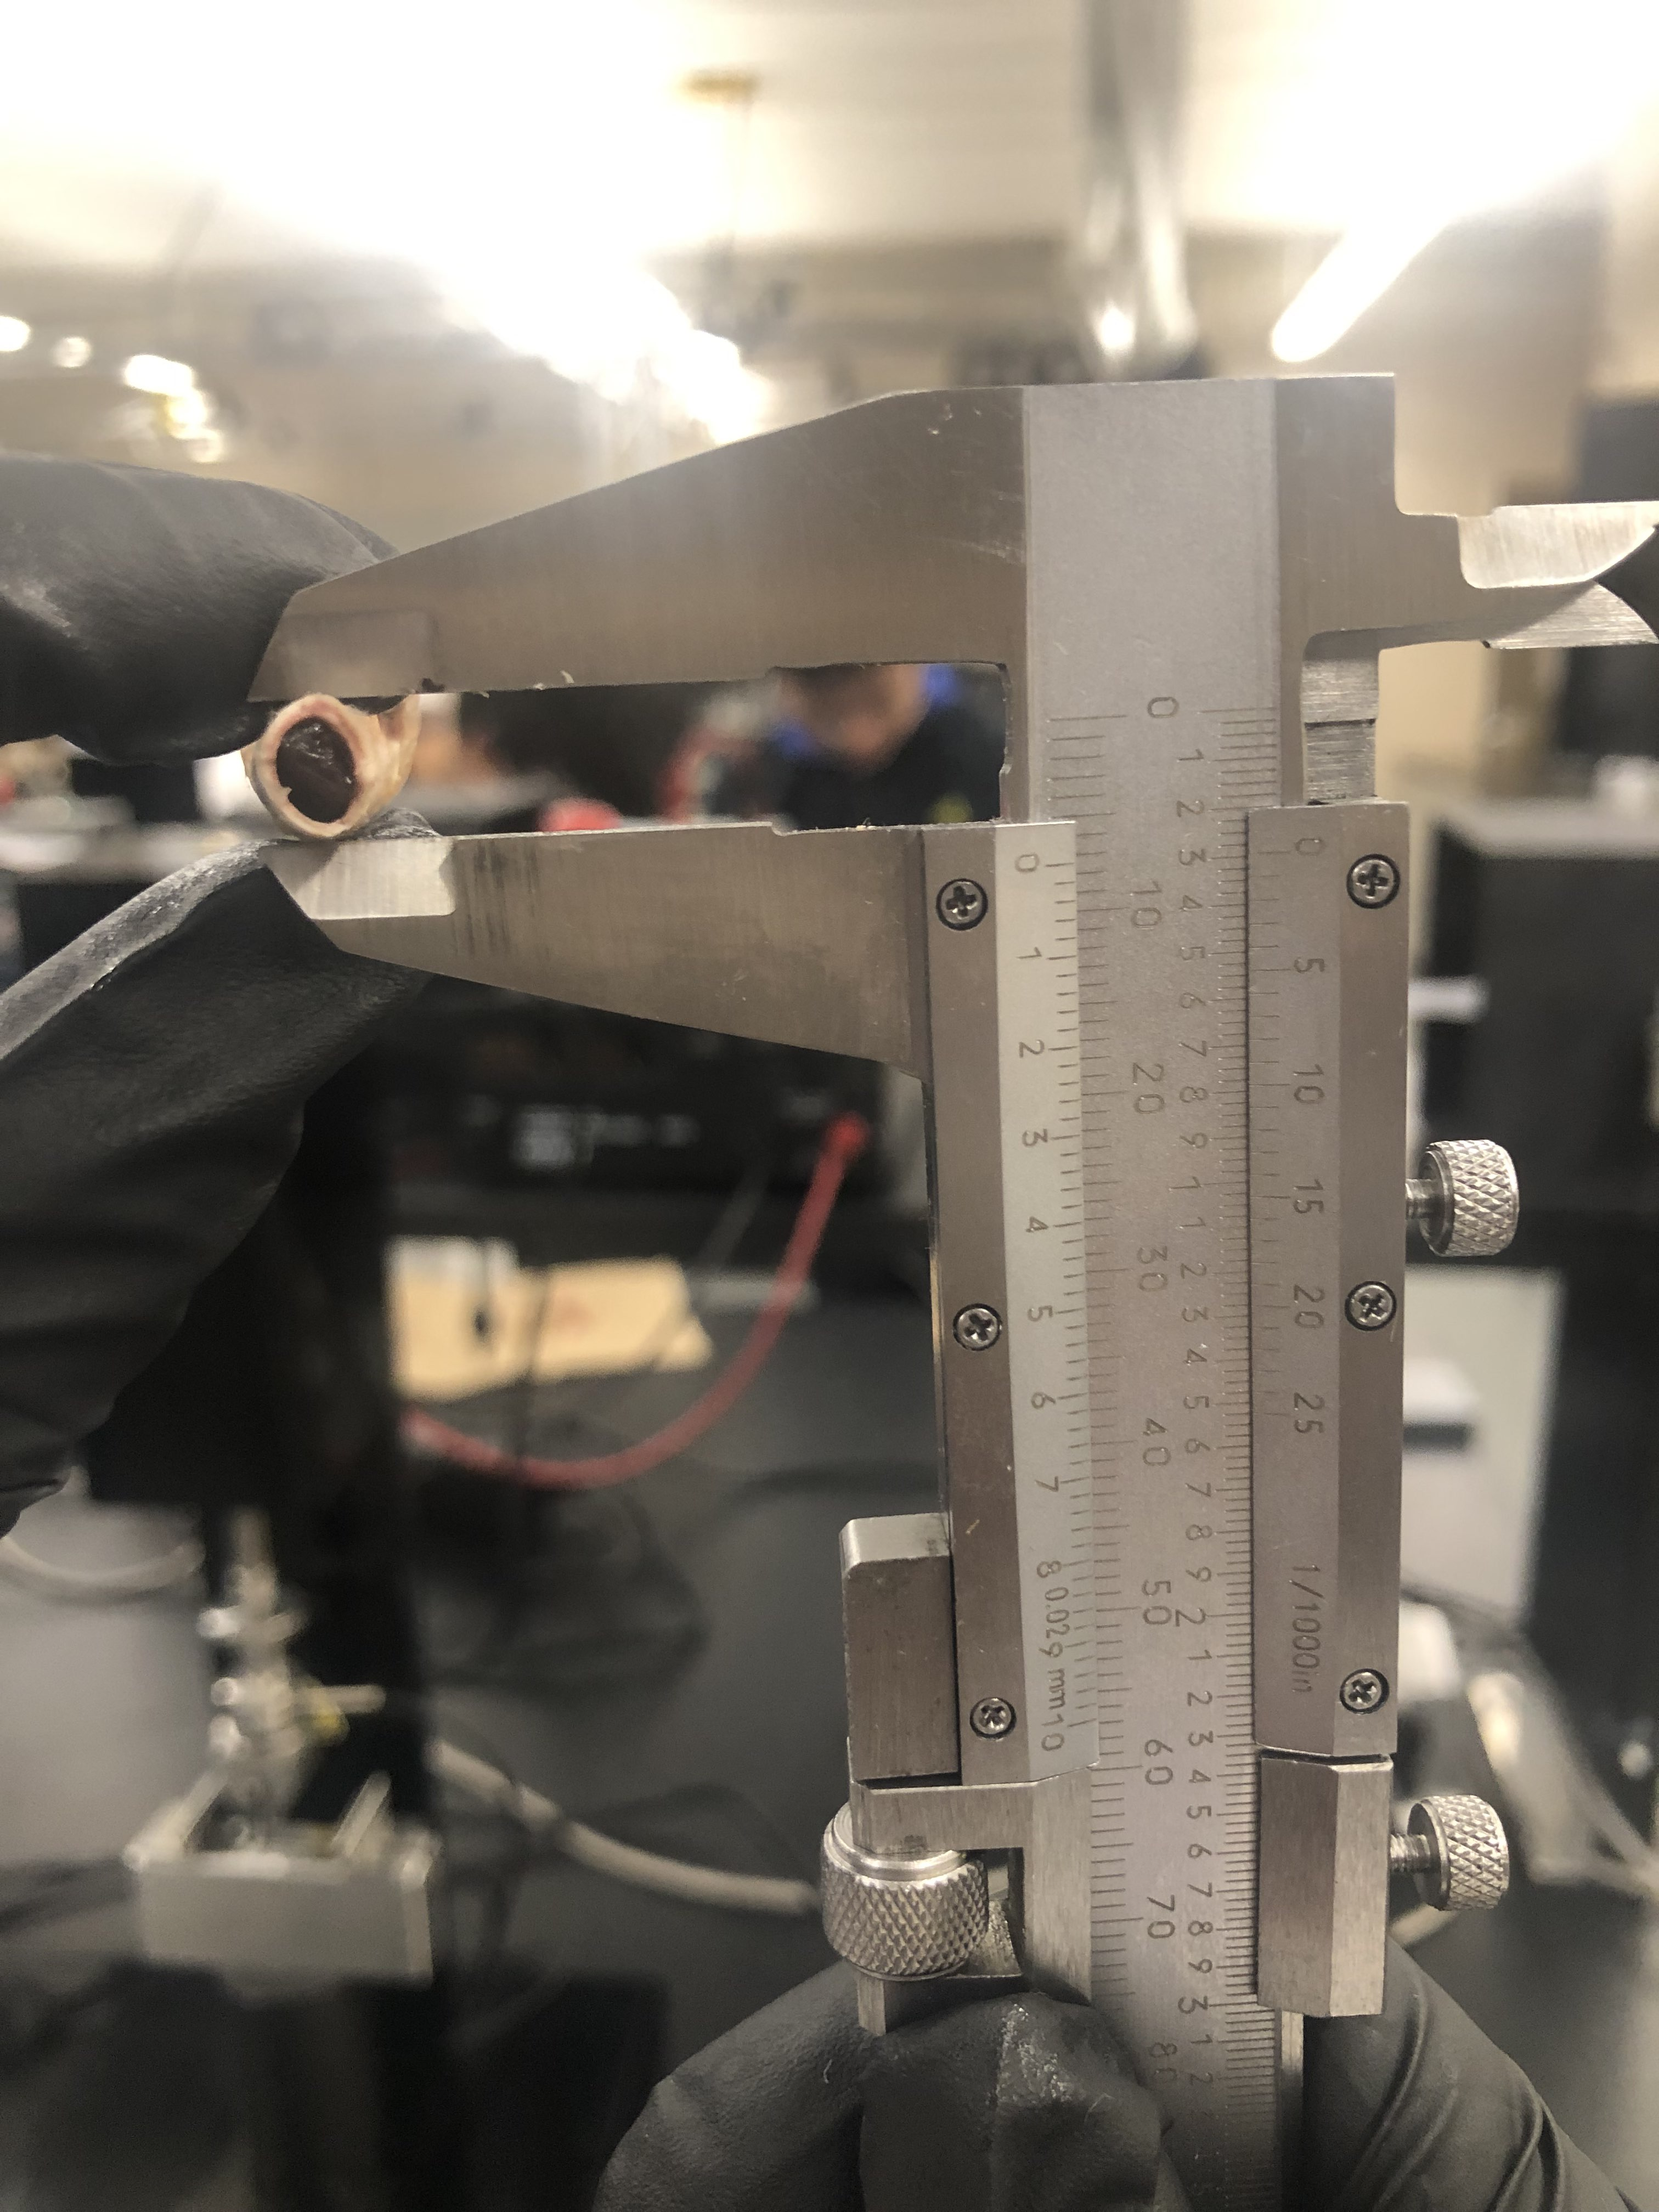
\includegraphics[width = 0.75\linewidth]{ulna_full.jpg}}
                \caption{Cross-section photo of ulna taken with vernier caliper for scaling.}\label{ulna_full}
            \end{figure}

            Using Solidworks, a picture of the cross-section of ulna (Fig.~\ref{ulna_full}) was imported into a sketch layer in the front plane so that the coordinate system matched that of Fig.~\ref{ulna_measurements}. The picture was scaled to match real-life dimensions using the caliper markings, as seen in Fig.~\ref{ulna_scale}.
            \begin{figure}[htbp]
                \centerline{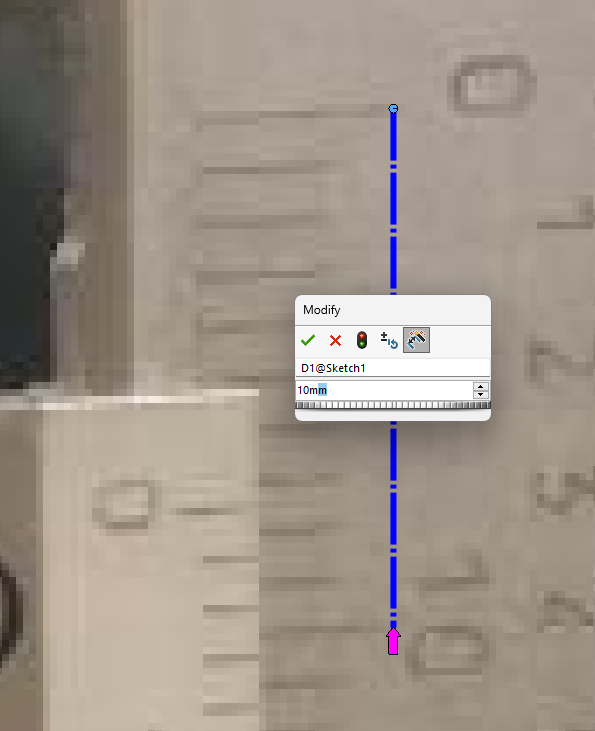
\includegraphics[width = 0.75\linewidth]{ulna_scale.png}}
                \caption{Screenshot of scaling process in Solidworks.}\label{ulna_scale}
            \end{figure}

            Then, using the spline tool, the cross-sectional area of the bone was outlined, as seen in Fig.~\ref{ulna_spline}. 
            \begin{figure}[htbp]
                \centerline{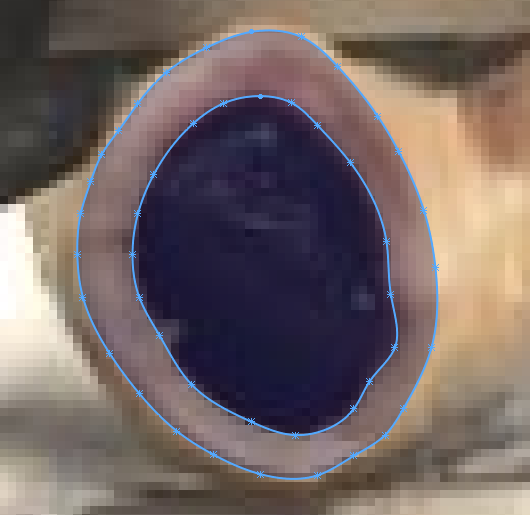
\includegraphics[width = 0.75\linewidth]{ulna_spline.png}}
                \caption{Screenshot of sketching process in Solidworks.}\label{ulna_spline}
            \end{figure}

            After confirming the sketch, it was extruded into a solid body (Fig.~\ref{ulna_extrude}).
            \begin{figure}[htbp]
                \centerline{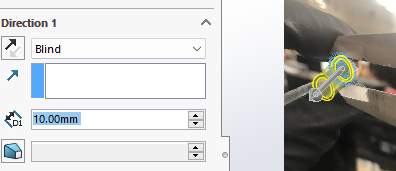
\includegraphics[width = \linewidth]{ulna_extrude.png}}
                \caption{Screenshot of extruding solid process in Solidworks.}\label{ulna_extrude}
            \end{figure}

            Finally, the cross-sectional face of the solid body was selected and section property analysis was ran on it; the results of the analysis can be seen in Fig.~\ref{ulna_section}. \(I_{xx} = 7.123\times10^{-11}\ \text{m}^4\)  was selected as the appropriate MOI for the bending setup as bending occurred about the x-axis.
            \begin{figure}[htbp]
                \centerline{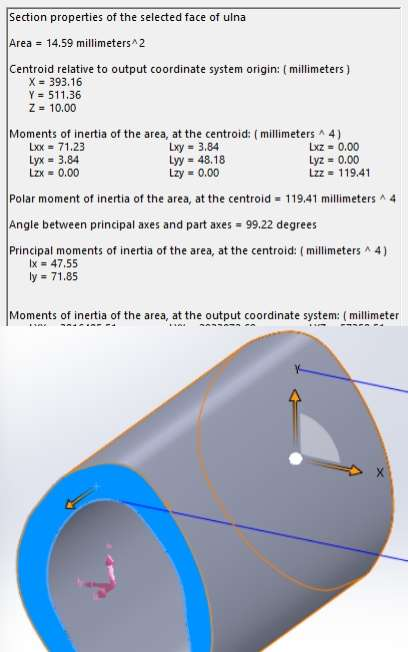
\includegraphics[width = \linewidth]{ulna_section.jpg}}
                \caption{Results of section property analysis on ulna.}\label{ulna_section}
            \end{figure}
            
\end{document}